\documentclass[conference]{IEEEtran}
\IEEEoverridecommandlockouts

\usepackage{cite}
\usepackage{amsmath,amssymb}
\usepackage{graphicx}
\usepackage{booktabs}
\usepackage{array}
\usepackage{xcolor}
\usepackage{url}
\usepackage[T1]{fontenc}

\graphicspath{{figures/}}

% consistent small-caps state names
\newcommand{\stt}[1]{\textsc{#1}}

\begin{document}

\title{Learning to Sense and React to Leg Entanglement on a Quadruped:\\
A Multi-Task Causal TCN Detector with Per-Leg Severity Estimation\\
and a Safety-Gated Recovery State Machine}

\author{\IEEEauthorblockN{Saurav Gupta}
\IEEEauthorblockA{\textit{Autonomous Systems Research}\\
\textit{Unitree Go2 Deployment Study}\\
sauravgupta1375@gmail.com}}

\maketitle

\begin{abstract}
Legged robots operating in cluttered or human environments can snag a leg on a
wire, net, or hand. Such entanglements are difficult to perceive with exteroceptive
sensors and, if undetected, precipitate stumbles or falls. We present a
proprioception-only system for a Unitree Go2 quadruped that predicts, at every
control step, \emph{whether} a leg is entangled, \emph{which} leg
(front-right/front-left/rear-right/rear-left), and \emph{how severe} the
entanglement is on a calibrated $0$--$1$ scale. The detector is a multi-task
causal Temporal Convolutional Network (TCN) operating on a $0.40$\,s sliding
window of $60$ proprioceptive channels; because it uses only the last-timestep
embedding of a strictly left-padded network, the offline-validated model is the
same computation that runs online. On a $25$-recording dataset with
leave-one-recording-out cross-validation the detector attains a detection
F1 of $0.807 \pm 0.142$, and on a held-out test split it reaches F1$=0.809$,
ROC-AUC$=0.956$, and per-leg exact-match$=0.908$, substantially exceeding a
rule-based thigh-torque baseline evaluated under the same protocol. Severity is
estimated without ground-truth labels through a physics-grounded, calibrated
index. The detector is exported to ONNX and runs at a mean of $0.99$\,ms per
window (p95 $1.24$\,ms) on a single CPU thread, within the $2$\,ms budget at
$500$\,Hz, and reproduces the research pipeline to $\approx\!10^{-6}$. We further
describe a ROS\,2 recovery subsystem: a pure, unit-tested finite-state machine
whose recovery state is driven by a detector-aware strategy manager that selects
among verified high-level Sport-API motions in a closed loop. We report what is
experimentally verified (detection, calibration, latency, functional recovery
logic) and are explicit about what remains an engineering assumption pending
real-robot trials (the physical efficacy, directions, and magnitudes of the
recovery motions). The recovery layer therefore ships disabled by default.
\end{abstract}

\begin{IEEEkeywords}
Legged robots, proprioception, entanglement detection, temporal convolutional
networks, multi-task learning, fault recovery, ROS\,2, Unitree Go2.
\end{IEEEkeywords}

\section{Introduction}
\IEEEPARstart{Q}{uadruped} robots increasingly operate in environments littered
with thin, compliant obstacles---cables, netting, vegetation, tethers---and, in
teleoperation or inspection settings, may have a leg physically grabbed. When a
leg becomes \emph{entangled}, the gait continues to command motions that fight the
constraint, quickly degrading balance and, in the worst case, causing a fall.
Detecting the snag early, localizing it to a specific leg, and estimating its
severity would let a controller intervene before the situation becomes
unrecoverable.

Entanglement is a poor fit for exteroceptive perception. Thin wires and
transparent lines are hard to segment, self-occlusion hides the affected leg, and
cameras add latency and failure modes. Proprioception, by contrast, is already
streamed by the robot at high rate: joint positions, velocities and torques, foot
contact forces, and the inertial measurement unit (IMU) all respond immediately
when a leg is held back. The signature, however, is subtle---on our platform a
rear-thigh torque dip of only $1$--$2$\,N$\cdot$m---and is easily confused with
normal gait variation, standing, or the rigid ``locked'' stance the robot adopts
after standing up. A single hand-tuned threshold is therefore brittle.

We take a learning approach. Our central object is a compact multi-task causal
TCN that, from proprioception alone, jointly answers three questions at every
timestep: detection (is any leg entangled?), attribution (which leg?), and
severity (how strongly?). The three outputs are complementary---attribution tells
a recovery policy \emph{where} to act and severity tells it \emph{how
aggressively}---and, to our knowledge, per-leg severity estimation for
entanglement has not previously been reported for a commercial quadruped.

This paper makes four contributions.
\begin{enumerate}
\item A multi-task causal TCN detector for leg entanglement that predicts
detection, per-leg attribution, and a per-leg severity index from a $0.40$\,s
proprioceptive window, with a strictly causal architecture that makes the
offline-validated model identical to the online one.
\item A physics-grounded, calibrated $0$--$1$ intensity index that requires no
ground-truth severity labels, combining a Mahalanobis deviation from the walking
manifold with a resistive-effort term and gated by the per-leg probability.
\item A rigorous evaluation---leave-one-recording-out cross-validation, a
leakage-safe held-out split, probability calibration, feature ablation, and a
documented before/after study of four field-observed deployment failures---together
with a CPU-only ONNX runtime that matches the research pipeline to $\approx\!10^{-6}$
and meets the real-time budget.
\item A ROS\,2 recovery subsystem built as a pure, unit-tested finite-state
machine with a detector-aware strategy manager that selects among verified
high-level Sport-API motions in a closed loop, with safety gating and a dry-run
default.
\end{enumerate}
Throughout, we separate verified experimental results from engineering assumptions;
in particular, the \emph{disentanglement efficacy} of the recovery motions is not
yet hardware-validated and is stated as such.

\section{Related Work}
The closest prior work is Yim \emph{et al.}~\cite{yim2023entanglement}, who address
proprioceptive sensing and reaction for walking among entanglements. Their system
detects entanglement from proprioception and executes a disentanglement maneuver
during the swing phase as the affected leg advances, succeeding in $14$ of $16$
laboratory trials across obstacle stiffnesses and geometries. Their detector and
reaction are primarily rule-based and tightly coupled to the swing-phase timing of
the gait. Our work differs along three axes. First, detection is
\emph{learning-based and temporal}: a causal TCN integrates a $0.40$\,s history
rather than reacting to an instantaneous threshold, which we found necessary given
the subtlety of the signature on our platform. Second, we produce
\emph{structured} outputs---per-leg attribution and a calibrated severity
index---rather than a single binary reaction trigger. Third, we decouple
\emph{perception from actuation}: the detector publishes a state estimate that a
separate, safety-gated recovery state machine consumes, so recovery is not tied to
a particular gait phase and can be validated in a dry-run mode before any motion is
commanded.

Proprioceptive learning for legged robots is well established for locomotion and
state estimation. End-to-end reinforcement learning produces robust gaits from
proprioception~\cite{hwangbo2019learning,lee2020learning}, and probabilistic
contact estimation infers foot contact and impacts from joint and inertial
signals~\cite{camurri2017contact,bledt2018contact}. Entanglement detection is
related but distinct: the fault is an external kinematic constraint on a swinging
or standing leg rather than a contact or balance event, and it must be localized
and graded. Our temporal backbone follows the dilated causal convolution
literature~\cite{oord2016wavenet,bai2018tcn}, which shows that convolutional
sequence models match or exceed recurrent networks while remaining causal and
cheap to run. Because a downstream controller must reason about the detector's
confidence, we apply temperature scaling~\cite{guo2017calibration} and evaluate
calibration explicitly~\cite{niculescu2005predicting}. The runtime is built on
ROS\,2~\cite{macenski2022ros2} and the Unitree Sport-Mode
API~\cite{unitree_ros2,unitree_go2}, with inference deployed through ONNX
Runtime~\cite{onnxruntime}.

\section{System Overview}
\begin{figure*}[t]
  \centering
  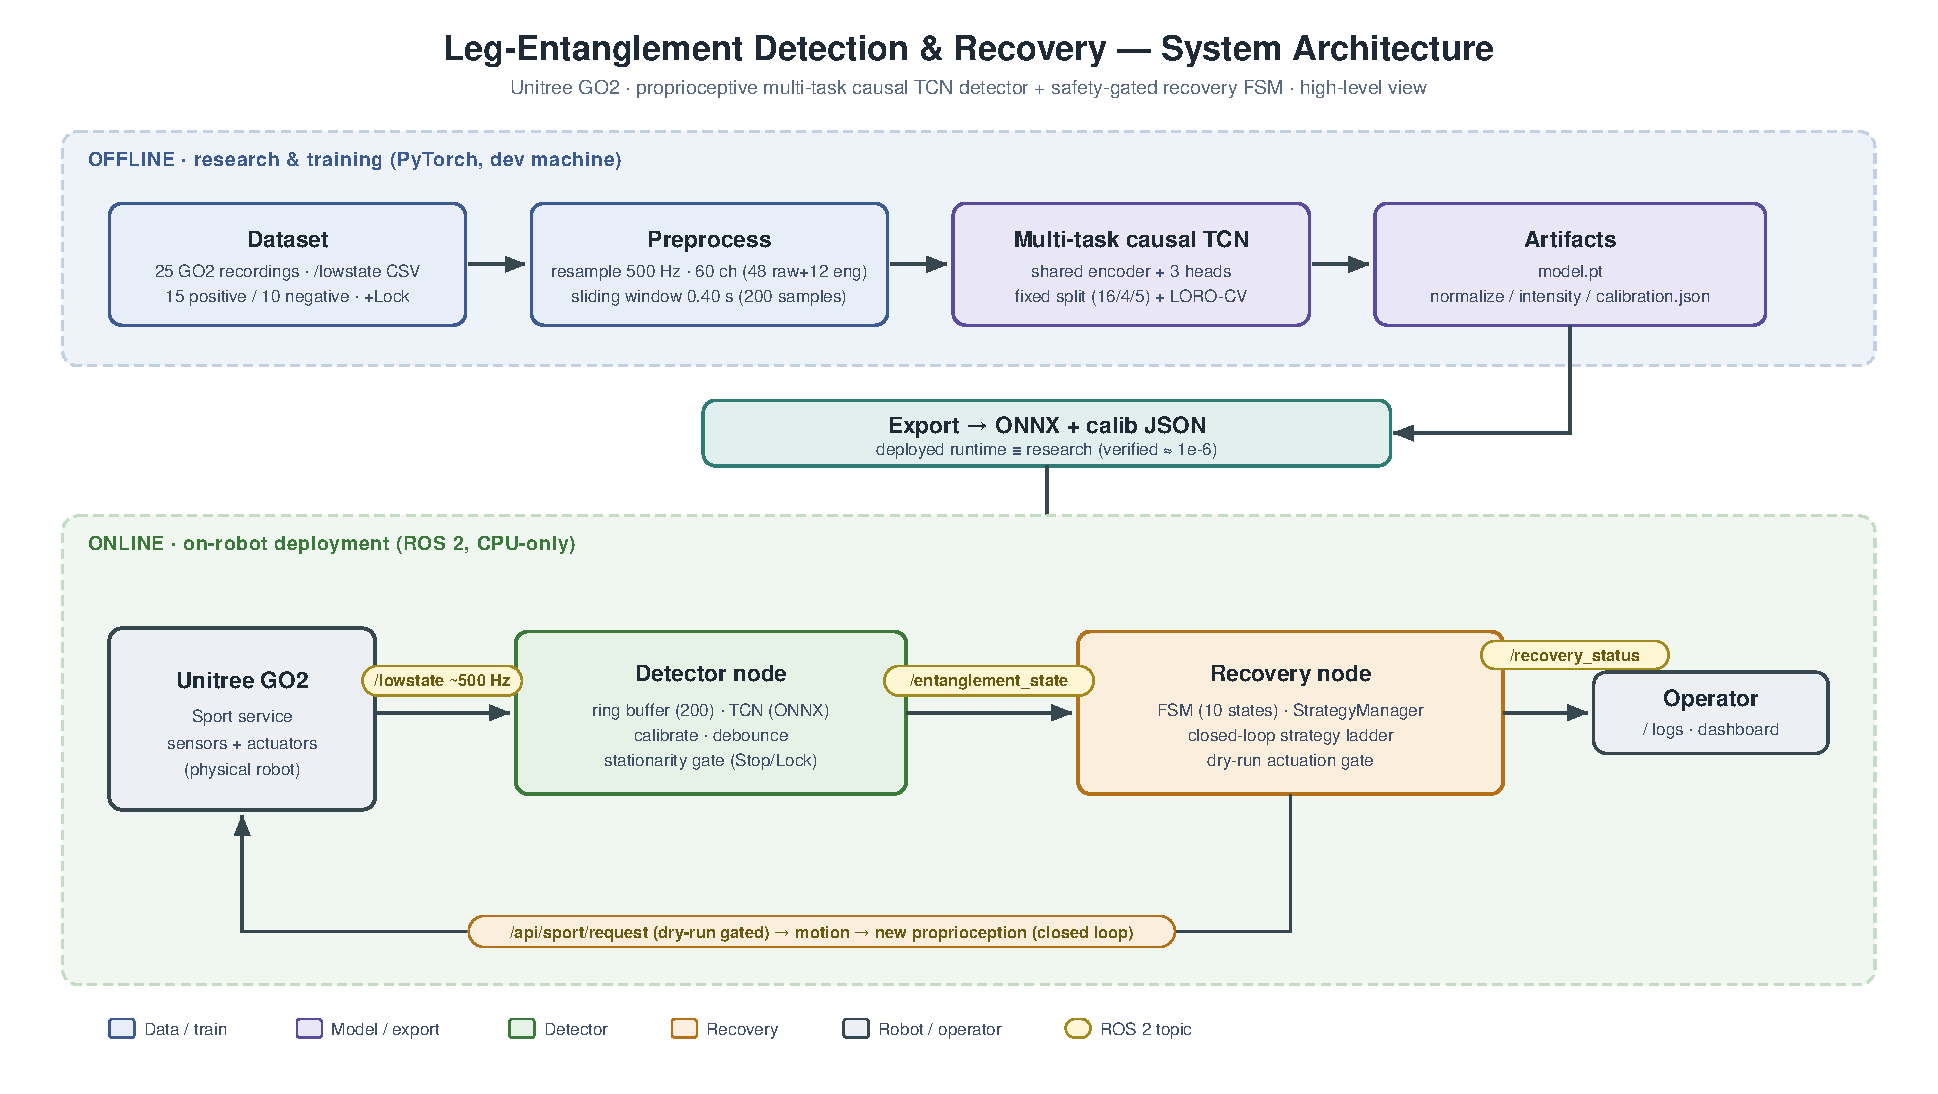
\includegraphics[width=\textwidth]{architecture_highlevel.pdf}
  \caption{System architecture. Offline (top): a labeled proprioceptive dataset is
  preprocessed into $60$-channel windows and used to train a multi-task causal TCN,
  whose artifacts are exported to ONNX. Online (bottom): on the Go2, a detector node
  consumes \texttt{/lowstate}, publishes \texttt{/entanglement\_state}, and a
  recovery node consumes that estimate and commands verified Sport-API motions in a
  closed loop, gated to dry-run by default.}
  \label{fig:arch}
\end{figure*}

Fig.~\ref{fig:arch} summarizes the system. It has an offline half and an online
half that share a single data contract. Offline, in PyTorch~\cite{paszke2019pytorch},
raw recordings are timestamp-normalized, label-merged, resampled to a common rate,
converted into $60$-channel windows, and used to train and evaluate the detector;
the trained weights and calibration parameters are exported once. Online, on the
robot, a ROS\,2 detector node wraps the exported model behind the same
preprocessing and publishes an entanglement state estimate; a separate recovery
node consumes that estimate and, when enabled, drives the robot through a recovery
sequence. The research and deployment code paths are an intentional mirror rather
than a duplication: the research side uses pandas/PyTorch and is the source of
truth for training, while the robot side is numpy\,+\,ONNX for a Python-3.8, CPU-only
target, and the two are checked to agree numerically (Section~\ref{sec:runtime}).

\section{Dataset Collection}
\label{sec:dataset}
\begin{table}[t]
\centering
\caption{Dataset composition ($25$ recordings, $159{,}001$ rows,
$409$--$960$\,Hz, no missing values).}
\label{tab:dataset}
\footnotesize
\begin{tabular}{@{}lccl@{}}
\toprule
Scenario & \#Rec. & Affected & Interaction \\
\midrule
\texttt{back\_both}        & 2 & RR, RL & wire \\
\texttt{back\_left}        & 3 & RL     & hand / wire \\
\texttt{back\_right}       & 3 & RR     & hand / wire \\
\texttt{front\_both}       & 2 & FR, FL & wire \\
\texttt{front\_left}       & 2 & FL     & hand \\
\texttt{front\_right}$^{\dagger}$ & 1 & FR & wire \\
\texttt{back\_right}$^{\dagger}$ & 2 & RR & wire, at rest \\
\midrule
\texttt{walking}           & 5 & ---    & normal gait \\
\texttt{stop}              & 3 & ---    & standing \\
\texttt{lock\_stop}$^{\dagger}$ & 1 & --- & stand-up / Lock \\
\texttt{walk\_stop\_back}$^{\dagger}$ & 1 & --- & backward gait \\
\midrule
\textbf{Total} & \textbf{25} & \multicolumn{2}{l}{\textbf{15 pos.\ / 10 neg.}}\\
\bottomrule
\end{tabular}
\\[2pt]
\raggedright\footnotesize $^{\dagger}$ Five recordings added in the second data
round from on-robot deployment, including the first dedicated front-right event and
the rigid ``Lock'' stance.
\end{table}

Data were collected on a Unitree Go2 by streaming the \texttt{/lowstate} topic. Each
recording contains a single scripted interaction. Table~\ref{tab:dataset} lists the
scenarios. In total there are $25$ recordings and $159{,}001$ rows, with a
per-file sample rate that varies from $409$ to $960$\,Hz (median $\approx\!536$\,Hz)
because logging is not perfectly periodic; this variability motivates the resampling
step in Section~\ref{sec:features}. Each row has $51$ columns: a timestamp, $36$
motor channels (position $q$, velocity $\dot q$, and estimated torque $\tau$ for the
hip, thigh, and calf of each of the four legs), four foot-force channels, an IMU
block, and a \texttt{Status} label.

\emph{Labeling.} Two facts shape the labels. First, the entangled leg is encoded in
the recording's filename (e.g.\ \texttt{back\_left}$\rightarrow$RL,
\texttt{front\_both}$\rightarrow$\{FR,FL\}), not in the per-row label; the per-row
\texttt{Status} carries only the temporal phase
(\texttt{Walking}, \texttt{Entangled}, \texttt{Stop}, \texttt{Lock}, or blank).
Second, each positive recording contains exactly one contiguous entangled segment,
which we treat as the event. This yields $15$ positive and $10$ negative recordings.
A key negative class is \texttt{Lock}: the rigid, high-stiffness stance the robot
holds immediately after standing up. Early field trials showed the detector firing
during this stance, so two recordings containing \texttt{Lock} and backward walking
were added specifically to teach the model these hard negatives. \texttt{Lock} is
handled as an ordinary negative (the same class as \texttt{Stop}); no new output head
was introduced.

\emph{Distribution and its consequences.} Fig.~\ref{fig:dataset} shows the class
composition. The affected-leg distribution is uneven: the front-right leg appears as
a positive in only three recordings, whereas the rear-right appears in seven. This
imbalance is a direct consequence of how the interactions were staged and, as we
show in Section~\ref{sec:results}, is the dominant driver of the front-right
precision trade-off and of the variance across cross-validation folds. It is the
clearest data-collection priority for future work.

\begin{figure*}[t]
  \centering
  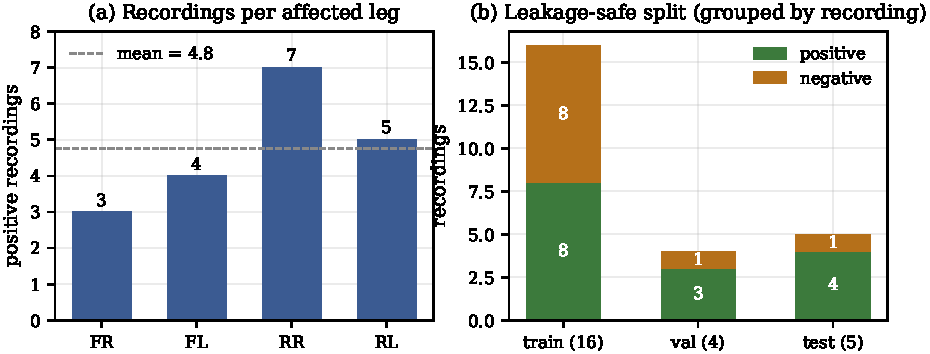
\includegraphics[width=\textwidth]{dataset_distribution.pdf}
  \caption{Dataset distribution. (a) Number of positive recordings in which each leg
  is the affected leg; the front-right leg is markedly under-represented. (b) The
  leakage-safe split, grouped by recording so that no window is shared across
  train/val/test.}
  \label{fig:dataset}
\end{figure*}

\section{Feature Engineering}
\label{sec:features}
Because the logging rate is non-uniform, every recording is first resampled to a
common $500$\,Hz grid---linear interpolation for continuous signals and
nearest-neighbor for the discrete \texttt{Status} label, which is never
interpolated. At $500$\,Hz one step is $2$\,ms, matching the robot's control cadence,
so that a fixed-length temporal filter means the same thing on every recording.

The model input is a $60$-channel window (Table~\ref{tab:features}). Forty-eight
channels are raw: the $36$ motor signals, the four foot forces, and eight IMU
channels (roll, pitch, three gyroscope and three accelerometer axes; yaw is dropped
as an unbounded integrator). Twelve channels are engineered physics features, three
per leg, designed to expose the mechanical signature of a leg being held back:
$\texttt{thigh\_tau\_down}=\max(0,-\tau_{\text{thigh}})$ isolates the
resistive (downward) thigh torque; $\texttt{thigh\_down\_effort}=
\texttt{thigh\_tau\_down}/(|\dot q_{\text{thigh}}|+\varepsilon)$ with
$\varepsilon=0.05$ captures torque expended against little motion, the hallmark of a
constraint; and $\texttt{tau\_sum}=\sum_j|\tau_j|$ summarizes per-leg effort. These
features are cheap, interpretable, and (Section~\ref{sec:results}) measurably improve
generalization. Channels are z-score normalized using statistics fit on training rows
only.

\begin{table}[t]
\centering
\caption{Sixty-channel input representation.}
\label{tab:features}
\footnotesize
\begin{tabular}{@{}llc@{}}
\toprule
Group & Channels & Count \\
\midrule
Motor & $\{$FR,FL,RR,RL$\}\!\times\!\{$hip,thigh,calf$\}\!\times\!\{q,\dot q,\tau\}$ & 36 \\
Foot force & $\texttt{foot\_}\{$FL,FR,RL,RR$\}$ & 4 \\
IMU & roll, pitch, gyro$_{xyz}$, acc$_{xyz}$ (yaw dropped) & 8 \\
Engineered & per leg: 3 physics feat.\ (Sec.~\ref{sec:features}) & 12 \\
\midrule
\textbf{Total} & & \textbf{60} \\
\bottomrule
\end{tabular}
\end{table}

\emph{Windowing and labels.} Windows are $200$ samples ($0.40$\,s), roughly one trot
stride, with a hop of $25$ for training and $1$ for dense evaluation. A window is
labeled positive if at least half of its rows are \texttt{Entangled}; windows whose
entangled fraction falls in the ambiguous band $(0.2,0.5)$ are excluded from training
but kept for evaluation. When positive, the per-leg targets are set from the
recording's affected set; \texttt{Stop} and \texttt{Lock} windows are negatives. All
splits are grouped by recording so that no window straddles the train/test boundary.

\section{Machine Learning Pipeline}
\label{sec:ml}
\emph{Architecture.} The detector is a causal dilated TCN with a shared encoder and
three linear heads. A causal (left-padded) convolutional stem lifts the $60$ input
channels to a $64$-channel embedding, followed by five residual TCN blocks with
dilations $1,2,4,8,16$; each block applies two causal convolutions (kernel $3$) with
GELU activations and dropout $0.1$. The resulting receptive field is $127$ samples
($\approx\!254$\,ms), comfortably inside the window. Crucially, only the embedding at
the \emph{last} timestep is read out, and every convolution is left-padded, so the
prediction depends only on current and past samples. The three heads map the $64$-d
embedding to a detection logit, four per-leg logits, and four intensity outputs. The
network has $\approx\!136$k parameters.

\emph{Losses and imbalance.} Training minimizes
$\mathcal{L}=1.0\,\text{BCE}_{\text{det}}+1.0\,\text{BCE}_{\text{leg}}
+0.3\,\text{Huber}_{\text{int}}$, where the intensity term is masked to positive
windows. Class imbalance is handled by a weighted sampler that draws roughly balanced
batches and up-weights rare-leg windows, plus capped positive weights in the BCE
terms. Table~\ref{tab:hp} lists the configuration; all values are fixed in a single
configuration file that both training and evaluation import.

\begin{table}[t]
\centering
\caption{Model and training configuration.}
\label{tab:hp}
\small
\begin{tabular}{@{}ll@{}}
\toprule
Parameter & Value \\
\midrule
Window / hop (train, eval) & $200$ ($0.40$\,s) / $25$, $1$ \\
Resample rate & $500$\,Hz \\
Encoder width / blocks & $64$ / $5$ \\
Dilations, kernel, dropout & $1,2,4,8,16$; $3$; $0.1$ \\
Receptive field & $127$ samples ($254$\,ms) \\
Parameters & $\approx\!136$k \\
Loss weights (det/leg/int) & $1.0$ / $1.0$ / $0.3$ \\
Optimizer & AdamW~\cite{loshchilov2019adamw}, lr $10^{-3}$, wd $10^{-4}$ \\
Schedule / batch / epochs & cosine / $256$ / $30$ \\
Sampler & class-balanced, rare-leg up-weighted \\
Seed & $1234$ \\
\bottomrule
\end{tabular}
\end{table}

\emph{Severity without labels.} No ground-truth severity exists, so we define a
physics-grounded index per leg,
\[
I_{\text{leg}} = g_{\text{leg}}\cdot\sqrt{d_{\text{leg}}\cdot r_{\text{leg}}},
\]
where $d_{\text{leg}}$ is a calibrated Mahalanobis deviation of the window's per-leg
feature vector from the \emph{Walking} distribution (mean and covariance fit on
training walking windows only), $r_{\text{leg}}$ is the calibrated resistive effort
$\text{mean}\big(\max(0,-\tau_{\text{thigh}})/(|\dot q_{\text{thigh}}|+\varepsilon)\big)$,
and $g_{\text{leg}}$ is the per-leg probability, which gates the index to
$\approx\!0$ when the leg is not flagged. The deployed value blends this physics index
with the network's intensity head in equal parts. We report it as a
\emph{calibrated severity index}, not a measured force: it is near zero on
walking/standing/locked windows and rises monotonically with the strength of the
interaction (Section~\ref{sec:results}).

\emph{Model selection.} We chose a causal TCN over an LSTM/GRU and over a windowed
gradient-boosted classifier for three reasons: (i) causality is required for online
use and is structural in the TCN, not an afterthought; (ii) the dilated receptive
field spans a stride with a fixed, small per-window cost, which matters for the CPU
budget; and (iii) the shared encoder naturally supports the three heads. A
non-temporal baseline on window-averaged features and a rule-based thigh-torque
detector are used as comparisons in Section~\ref{sec:results}.

\section{Runtime Architecture}
\label{sec:runtime}
\begin{figure}[t]
  \centering
  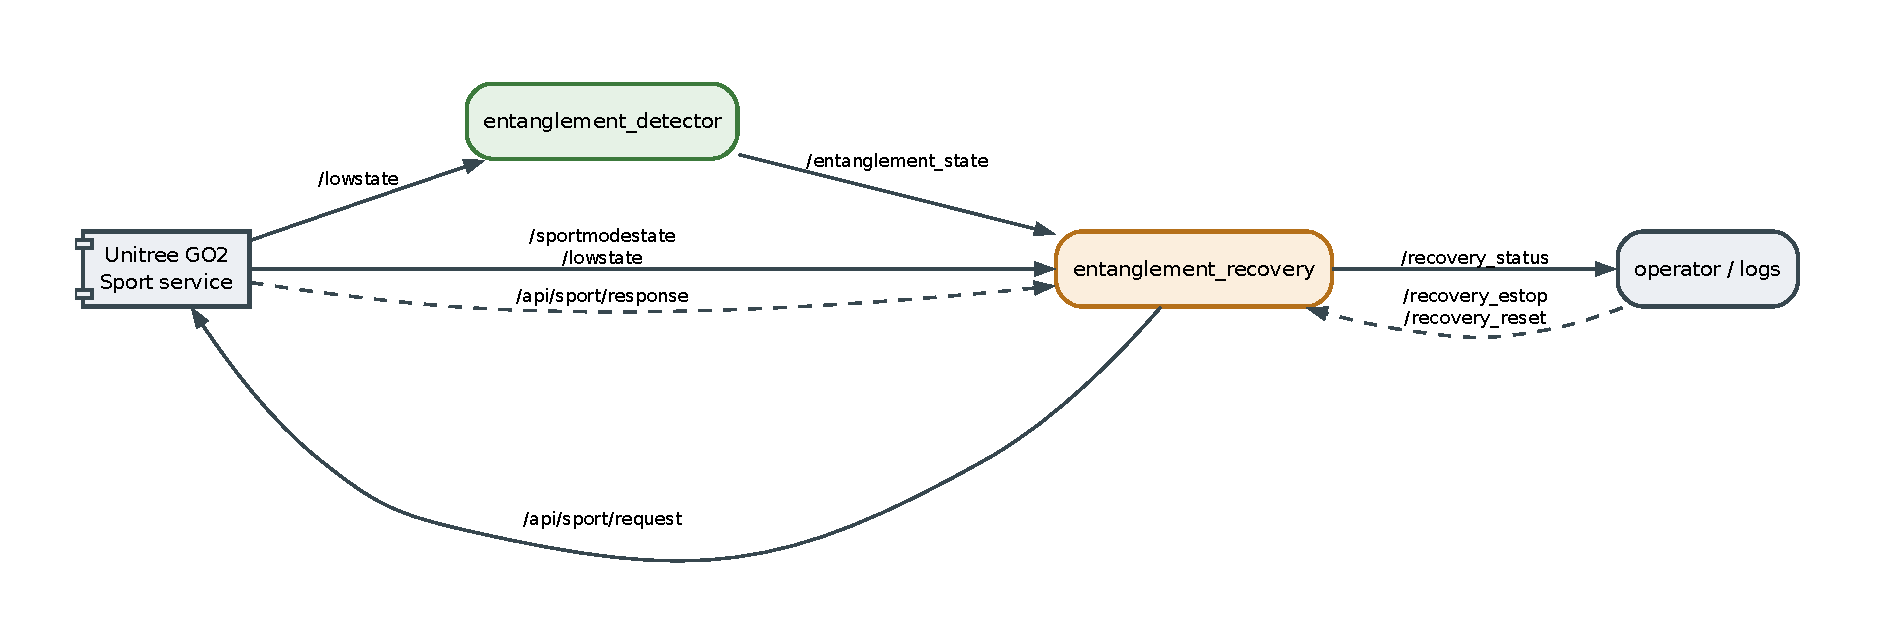
\includegraphics[width=\columnwidth]{ros_graph.pdf}
  \caption{ROS\,2 node graph. The detector consumes \texttt{/lowstate} and publishes
  \texttt{/entanglement\_state}; the recovery node additionally consumes robot
  telemetry and, when enabled, publishes Sport-API requests, exposing status and
  e-stop/reset topics. All robot-facing subscriptions use best-effort QoS.}
  \label{fig:ros}
\end{figure}

On the robot the detector is a ROS\,2 node (Fig.~\ref{fig:ros}) that subscribes to
\texttt{/lowstate} with best-effort QoS, adapts each message into the $48$ raw
signals, and feeds a streaming engine. The engine maintains a $200$-sample ring
buffer; once full, it builds the $60$-channel matrix, applies the saved
normalization, runs the ONNX forward pass, converts logits to probabilities, forms
the blended intensity, applies a raw-probability threshold with a $75$\,ms
time-based debounce, and finally names the alarm leg using per-leg thresholds. The
per-leg threshold for the rear-right leg is raised to $0.9$ to curb its false
positives; the others are $0.5$. The output message carries the debounced flag, a
temperature-calibrated confidence, four per-leg probabilities, four per-leg
intensities, and the alarm leg.

\emph{Stationarity gate.} A field failure was spurious firing when the robot stood up
into the rigid \texttt{Lock} stance or when stale entanglement context lingered after
the robot stopped. The engine therefore includes an edge-triggered stationarity gate:
when the mean absolute joint velocity stays below $0.30$\,rad/s for
$100$\,ms, the ring buffer and debounce counter are cleared once and a $300$\,ms
post-resume suppression window is armed to absorb gait re-acquisition transients. The
gate deliberately does \emph{not} blanket-suppress while stationary---entanglement
applied at rest must still be detectable---so suppression is edge-triggered and brief.
The gate is disabled by default in the research configuration to preserve exact
equivalence, and enabled on the robot.

\emph{Determinism between research and robot.} The deployment runtime is numpy-only
plus ONNX Runtime and is Python-3.8 compatible. We verified that it reproduces the
research pipeline's dense inference to $\approx\!10^{-6}$: the maximum absolute
difference over $3{,}052$ test windows is $3.8\times10^{-7}$ for the detection
probability, $6.3\times10^{-7}$ for per-leg probabilities, and $2.1\times10^{-7}$ for
intensity. This means the offline-validated numbers in Section~\ref{sec:results}
transfer to the robot without a reimplementation gap.

\section{Intelligent Recovery Framework}
\label{sec:recovery}
\begin{figure}[t]
  \centering
  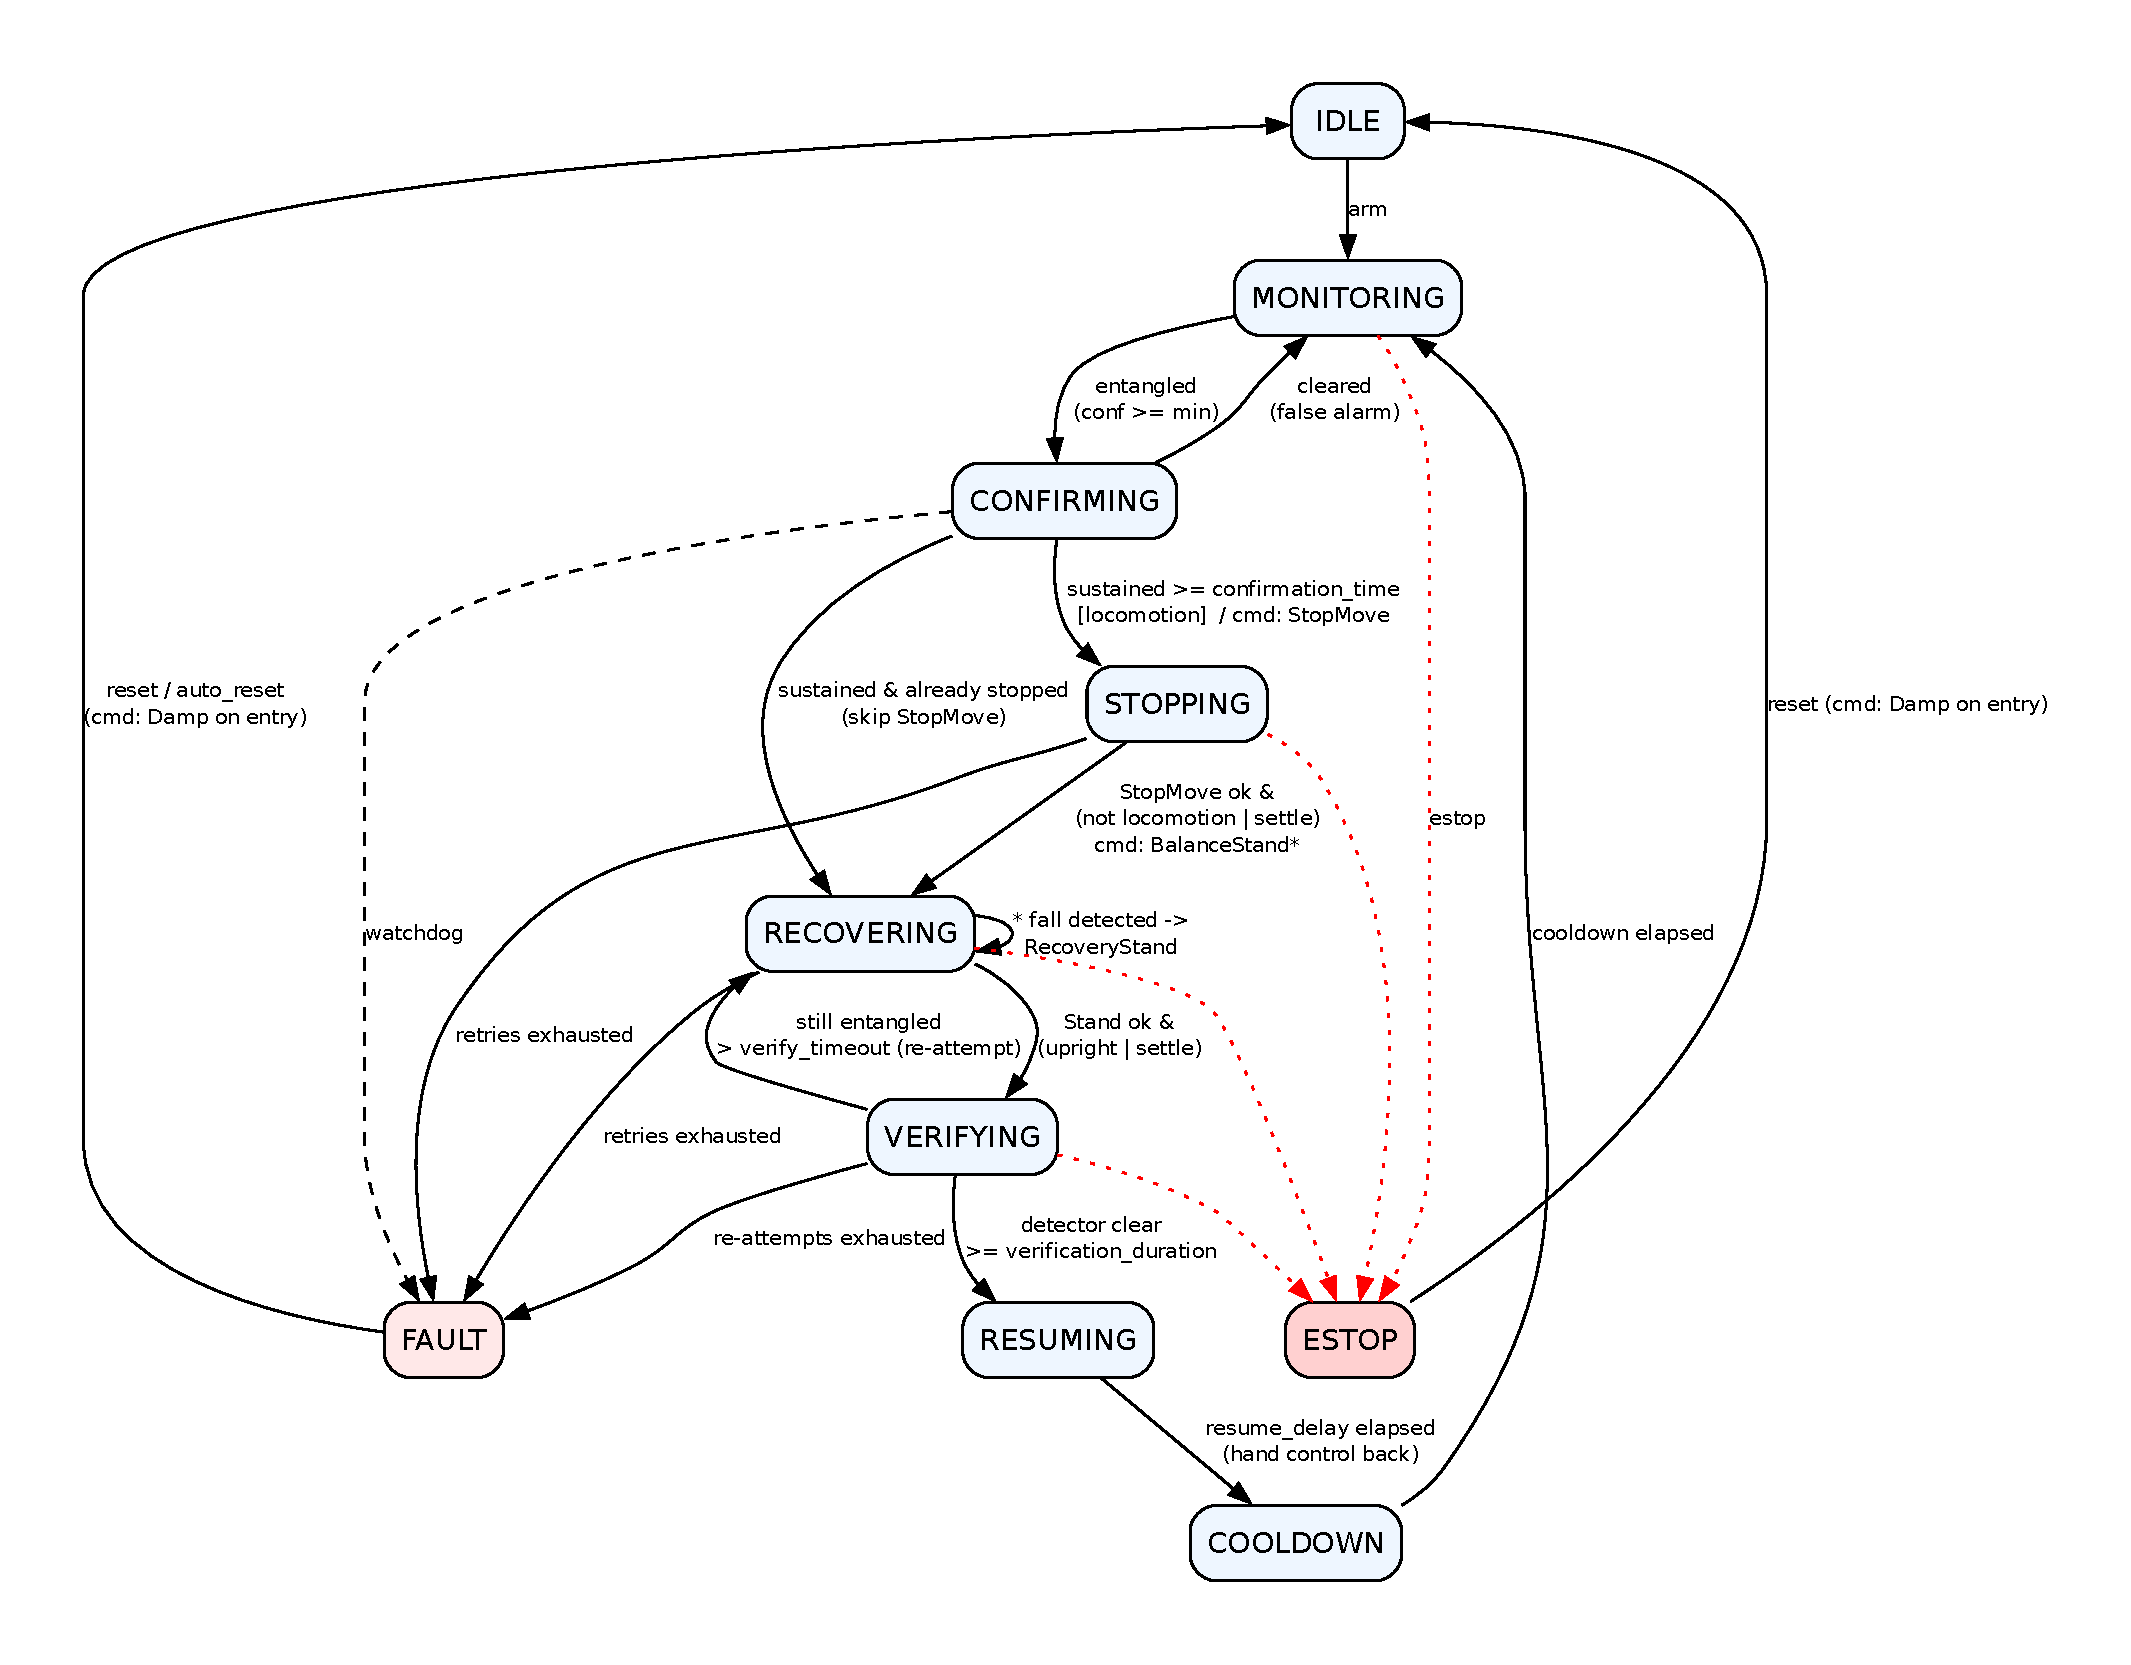
\includegraphics[width=\columnwidth]{recovery_state_machine.pdf}
  \caption{Recovery finite-state machine. The safety-critical logic is pure Python
  and unit-tested; \stt{estop} (damp) and \stt{fault} (damp) are reachable from any
  active state. The \stt{recovering} state delegates to the strategy manager.}
  \label{fig:fsm}
\end{figure}

The recovery subsystem is a separate ROS\,2 package that only \emph{subscribes} to the
detector's output; the detector is untouched. Its core is a pure finite-state machine
(Fig.~\ref{fig:fsm}) with no ROS dependencies, so the safety logic can be exercised
deterministically off-robot. Thin adapters connect it to ROS: one decodes robot
telemetry (\texttt{/sportmodestate} and \texttt{/lowstate}) into a posture, roll,
pitch, and battery estimate; one publishes Sport-API requests and tracks responses;
and an orchestrator ticks the machine at $50$\,Hz.

\emph{State machine.} The machine progresses
\stt{idle}$\rightarrow$\stt{monitoring}$\rightarrow$\stt{confirming}$\rightarrow$
\stt{stopping}$\rightarrow$\stt{recovering}$\rightarrow$\stt{verifying}$\rightarrow$
\stt{resuming}$\rightarrow$\stt{cooldown}. A detection must persist through
\stt{confirming} before any action, which rejects transient false alarms. If the
robot is already stopped, \stt{stopping} is skipped. \stt{verifying} closes the loop:
the machine watches the detector after a recovery attempt and either declares success
(the estimate stays clear for a fixed duration) or, on timeout, escalates to the next
strategy. Two states are reachable from anywhere: \stt{estop} on an external request
and \stt{fault} on repeated command failure or a per-state watchdog timeout; both
issue a damp (limp) command.

\emph{Detector-aware strategy manager.} The novelty of the recovery layer is that the
\stt{recovering} state is not a fixed sequence but a policy that consumes the full
detector output. Given the alarm leg, confidence, severity, posture, and battery, the
manager returns an ordered list of strategies to try (Table~\ref{tab:strategies}). If
the robot has fallen, it uses the fallen primitive (recovery-stand, gated on battery)
and otherwise the terminal safe action. If upright, it begins with the gentlest action
(balance-stand), then a weight shift away from the snagged corner, and---only when
confidence is high and severity is not extreme---small locomotion nudges (reverse,
side-step, rotate) whose directions are computed from the alarm leg. Extreme severity
deliberately \emph{suppresses} active locomotion to avoid thrashing a strongly stuck
leg, and motion magnitudes scale down as severity rises. The last resort is always an
emergency stop that damps the robot and hands control to the operator.

\begin{table}[t]
\centering
\caption{Recovery strategies and their verified Sport-API mapping. Kinematic effect
is verified against the SDK; disentanglement effect and motion direction/magnitude
are design assumptions (Section~\ref{sec:results}).}
\label{tab:strategies}
\footnotesize
\begin{tabular}{@{}lll@{}}
\toprule
Strategy & Trigger context & Sport API (id) \\
\midrule
balance\_stand   & upright, first/gentlest      & BalanceStand ($1002$) \\
weight\_shift    & upright, tilt off snag       & Euler ($1007$) \\
small\_reverse   & conf.\ high, sev.\ low        & Move ($1008$) \\
small\_sidestep  & conf.\ high, sev.\ low        & Move ($1008$) \\
rotate           & conf.\ high, sev.\ low        & Move ($1008$) \\
recovery\_stand  & fallen, battery ok           & RecoveryStand ($1006$) \\
emergency\_stop  & terminal / exhausted         & StopMove/Damp ($1003$/$1001$) \\
\bottomrule
\end{tabular}
\end{table}

\emph{Safety and design rationale.} Actuation is off by default: in dry-run the
orchestrator logs the command it \emph{would} send but transmits nothing, which lets
the entire pipeline be validated without moving the robot. Damp serves as the soft
e-stop and the terminal fault action. Recovery never re-enters while already active,
a cooldown follows each cycle, and a per-state watchdog forces a safe fault. We chose
high-level Sport-API primitives rather than low-level joint commands because the
former are documented and verifiable and keep the robot within its own balance
controller; the cost is that we cannot command an arbitrary joint trajectory to
extricate a leg, which is a genuine limitation we return to in
Section~\ref{sec:results}. The reason a weight shift precedes locomotion is that it is
the lowest-energy action that can reseat a lightly pinched foot without stepping into
the constraint; locomotion is escalated only when the detector is confident and the
snag is not severe.

\section{Experimental Setup}
\label{sec:setup}
All learning experiments use the grouped, leakage-safe split of
Fig.~\ref{fig:dataset}(b): $16$ recordings for training, $4$ for validation, and $5$
held out for test, with every window of a recording confined to one split. The
headline generalization metric is leave-one-recording-out (LORO) cross-validation
over the $15$ positive events, in which each positive recording is held out in turn
and scored with a threshold chosen from its own walking prefix. The detection
operating threshold on the fixed split is chosen on validation negatives for a low
per-window false-alarm rate and is reported alongside a post-hoc temperature and
per-leg thresholds; these post-hoc choices do not change the trained weights.
Baselines are a rule-based rear-thigh-torque detector and, for feature analysis, four
retrained channel-set ablations. Runtime latency is measured on a single CPU thread
with the ONNX backend by timing the per-window forward pass plus post-processing on a
test recording. Recovery logic is validated by $16$ finite-state-machine unit tests
and $3$ plan-runner unit tests that drive the pure machine with synthetic detection,
telemetry, and command results; no robot is in that loop.

\section{Results}
\label{sec:results}
\subsection{Detection}
Table~\ref{tab:detection} reports detection on the held-out test split. The TCN
attains F1$=0.809$, PR-AUC$=0.808$, ROC-AUC$=0.956$, and per-leg exact-match$=0.908$.
The rule-based baseline, evaluated identically, reaches F1$=0.222$: it is precise
when it fires ($0.735$) but recalls only $13\%$ of entangled windows, because it was
tuned for higher-amplitude signals than the subtle interactions in this dataset. The
confusion matrix (Fig.~\ref{fig:confusion}) shows the errors are roughly balanced
between missed and false detections rather than a single failure mode. The ROC and
precision-recall curves (Fig.~\ref{fig:rocpr}) confirm strong ranking performance
away from the clamped operating threshold.

\begin{table}[t]
\centering
\caption{Detection on the held-out test split (raw threshold $0.9999$).}
\label{tab:detection}
\small
\begin{tabular}{@{}lcc@{}}
\toprule
Metric & Causal TCN & Rule-based (thigh torque) \\
\midrule
Precision       & \textbf{0.799} & 0.735 \\
Recall          & \textbf{0.818} & 0.131 \\
F1              & \textbf{0.809} & 0.222 \\
PR-AUC          & \textbf{0.808} & 0.639 \\
ROC-AUC         & \textbf{0.956} & 0.830 \\
Leg exact-match & \textbf{0.908} & 0.106 \\
\bottomrule
\end{tabular}
\end{table}

\begin{figure}[t]
  \centering
  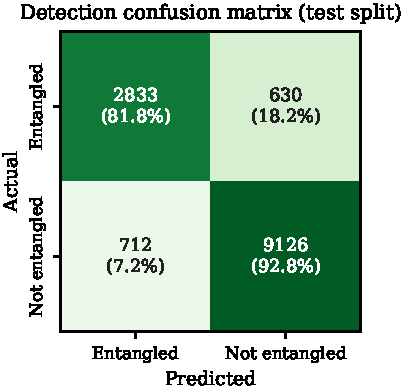
\includegraphics[width=0.86\columnwidth]{confusion_matrix.pdf}
  \caption{Detection confusion matrix on the test split (row-normalized), from
  $2{,}833$ true positives, $712$ false positives, $630$ false negatives, and
  $9{,}126$ true negatives.}
  \label{fig:confusion}
\end{figure}

\begin{figure}[t]
  \centering
  \begin{minipage}{0.49\columnwidth}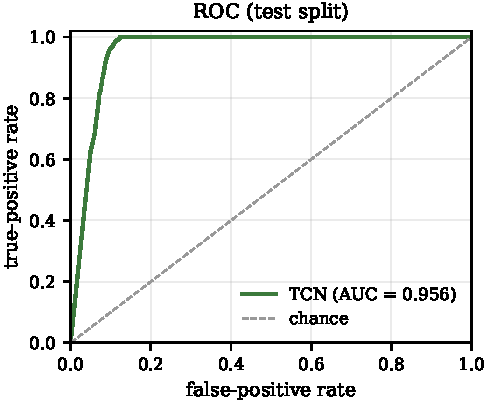
\includegraphics[width=\linewidth]{roc_curve.pdf}\end{minipage}\hfill
  \begin{minipage}{0.49\columnwidth}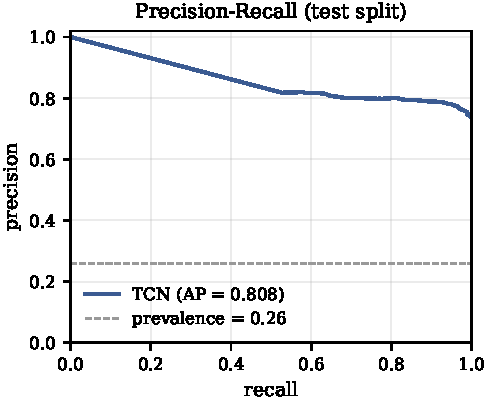
\includegraphics[width=\linewidth]{pr_curve.pdf}\end{minipage}
  \caption{ROC (left) and precision-recall (right) curves on the pooled test split,
  computed from the model's per-window scores.}
  \label{fig:rocpr}
\end{figure}

\subsection{Generalization}
LORO cross-validation (Fig.~\ref{fig:loro}) gives a detection
F1 of $0.807 \pm 0.142$ over $15$ folds, consistent with the fixed-split value and
indicating the split is representative rather than fortuitous. The weakest folds are
exactly the under-represented cases: the dedicated front-right recording and the two
rear-right ``stop/intensity'' recordings, whose interactions differ from the rest of
the corpus. This is the expected behavior of an honest per-recording protocol and
localizes where more data is needed.

\begin{figure*}[t]
  \centering
  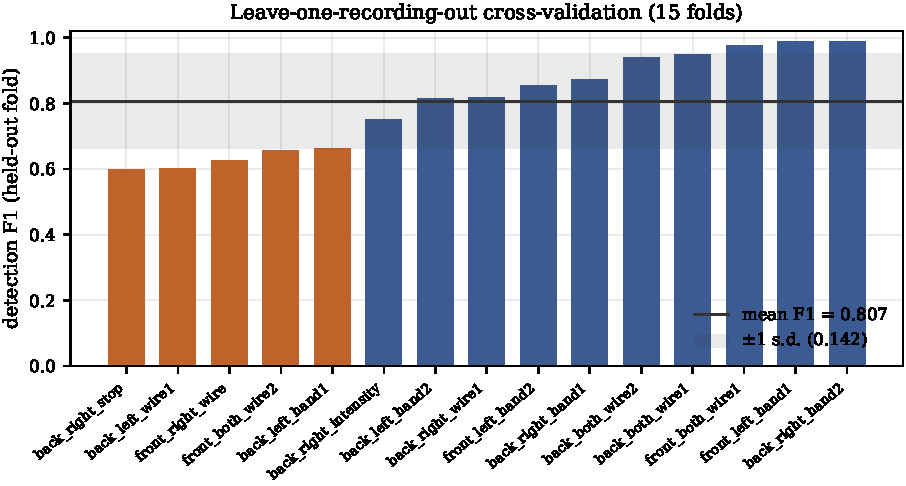
\includegraphics[width=\textwidth]{loro_folds.pdf}
  \caption{Leave-one-recording-out cross-validation. Each bar is the detection F1 when
  that recording is held out; the line and band are the mean and $\pm$one standard
  deviation. The weakest folds are the under-represented front-right and rear-right
  ``stop/intensity'' scenarios.}
  \label{fig:loro}
\end{figure*}

\subsection{Per-leg attribution and severity}
Per-leg scores on the test split (Fig.~\ref{fig:perleg}) are strong for the
well-represented legs (FL F1$=0.845$, RL F1$=0.823$) and weaker in precision for the
rear-right (F1$=0.700$) and front-right (F1$=0.636$, recall $1.0$, precision $0.47$).
The front-right precision is the direct cost of learning a dedicated front-right
signature from a single recording; recall remains perfect, and in deployment the
per-leg output is gated by the binary detection so the low precision does not, by
itself, raise the alarm rate. Qualitatively, the severity index behaves as designed:
Fig.~\ref{fig:timeline} shows a front-right event in which detection, the correct
per-leg probability, and the per-leg intensity all rise together at onset and decay at
release, while the other legs stay near zero.

\begin{figure}[t]
  \centering
  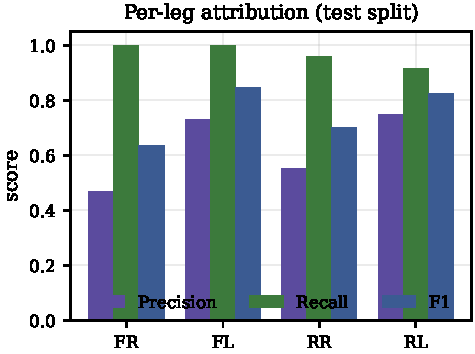
\includegraphics[width=\columnwidth]{per_leg_metrics.pdf}
  \caption{Per-leg attribution on the test split. The front-right leg trades precision
  for recall, reflecting its single training recording.}
  \label{fig:perleg}
\end{figure}

\begin{figure*}[t]
  \centering
  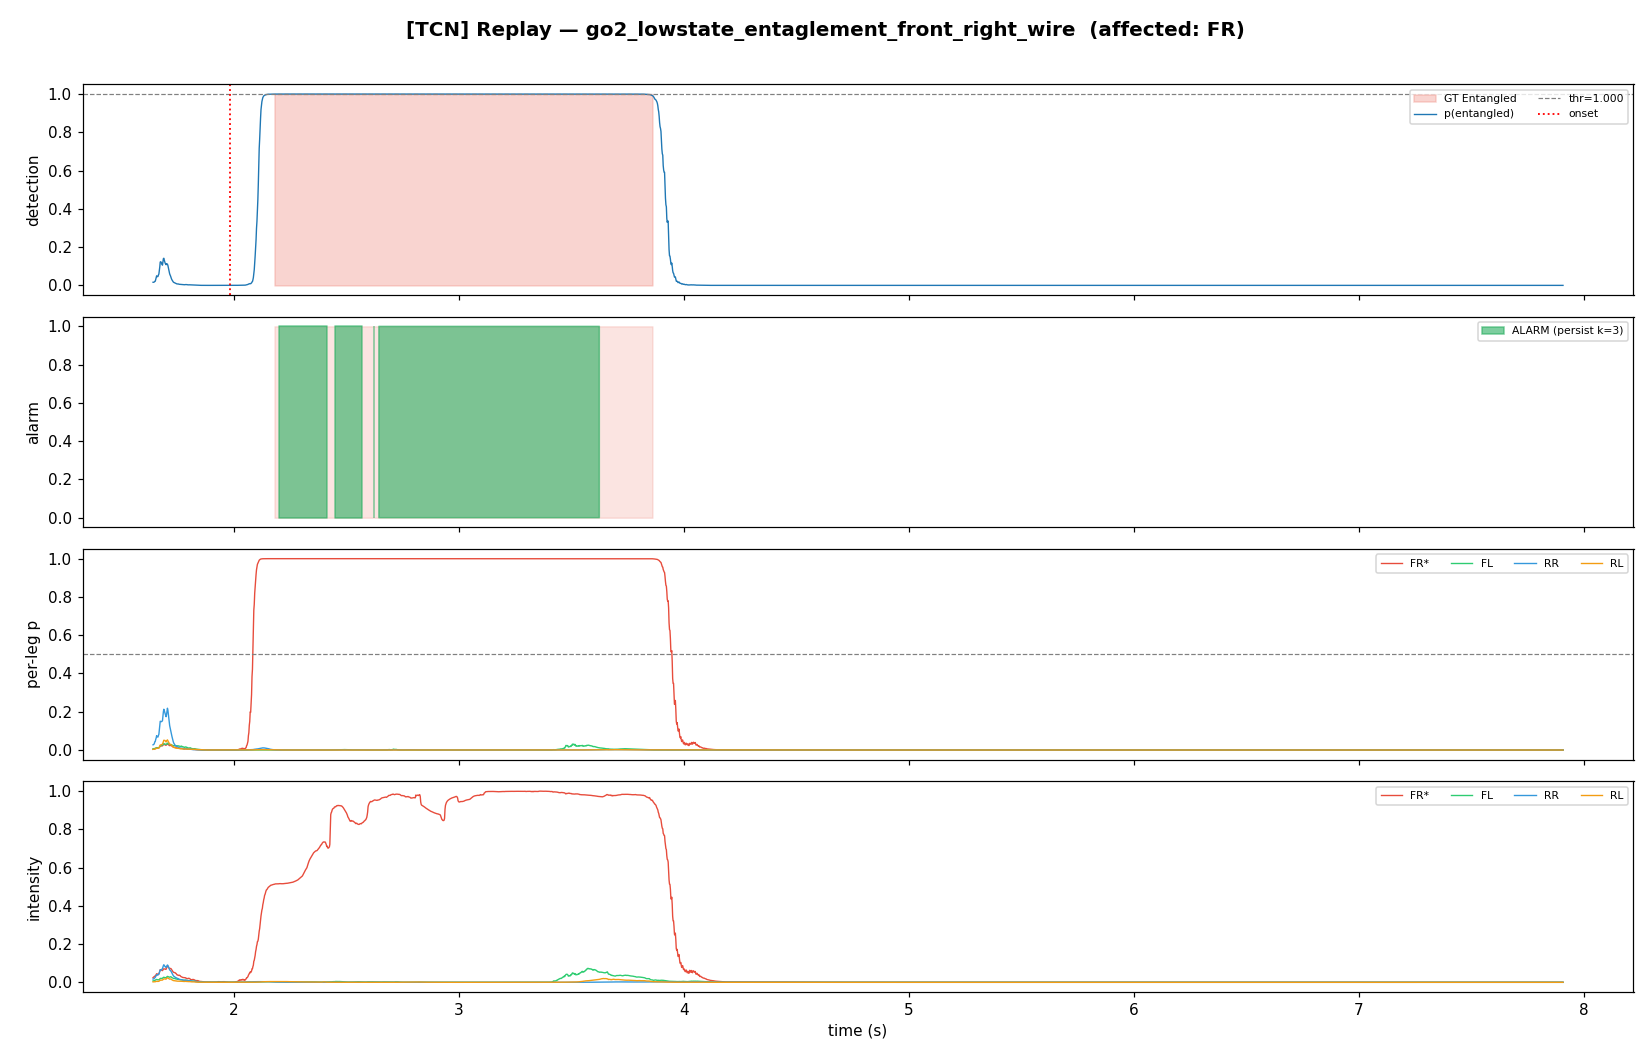
\includegraphics[width=\textwidth]{timeline_front_right.png}
  \caption{Detector output over time on a held-out-style front-right wire event.
  From top: detection probability with the ground-truth entangled ribbon; the
  debounced alarm; per-leg probability (front-right in red); and per-leg severity.
  All three outputs rise at onset, localize to the correct leg, and decay at release.}
  \label{fig:timeline}
\end{figure*}

\subsection{Calibration}
The raw detection probabilities are saturated---a large fraction sit at $1.0$---so the
false-alarm-rate threshold clamps at $0.9999$ and small confidence differences are
lost. Temperature scaling ($T=5.9$) de-saturates the distribution, which lets the
operating threshold move to a meaningful $0.963$, and modestly improves the Brier
score. Fig.~\ref{fig:reliability} shows the reliability diagram before and after
scaling. We note that scaling improves Brier and de-saturation but does not by itself
make the model perfectly calibrated; a downstream controller should treat the
calibrated confidence as a usable ordering rather than an exact probability.

\begin{figure}[t]
  \centering
  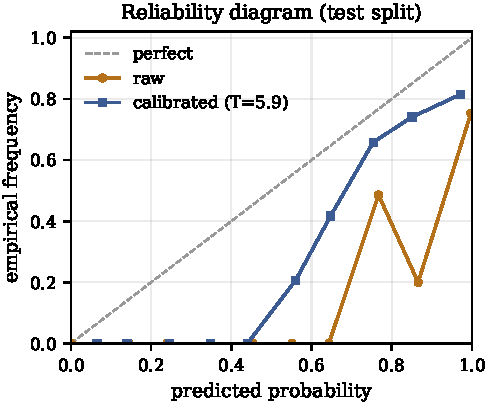
\includegraphics[width=0.86\columnwidth]{reliability_curve.pdf}
  \caption{Reliability diagram on the test split, raw versus temperature-calibrated.
  Scaling de-saturates the probability mass, enabling a meaningful operating
  threshold.}
  \label{fig:reliability}
\end{figure}

\subsection{Feature ablation}
Table~\ref{tab:ablation} reports LORO F1 for retrained channel-set variants. Raw
kinematics are essential (dropping them collapses performance), the engineered
channels help (raw+engineered $0.832$ vs.\ raw-only $0.799$), and the IMU is nearly
redundant for detection (no-IMU $0.833$ is statistically indistinguishable from the
full set). This suggests a leaner input is possible for tighter on-robot latency; we
retain the full set for robustness. This ablation is a feature-set study; it predates
the final data round and is reported as an architecture-level analysis.

\begin{table}[t]
\centering
\caption{Feature-set ablation (LORO F1, mean $\pm$ s.d.).}
\label{tab:ablation}
\small
\begin{tabular}{@{}lcc@{}}
\toprule
Channel set & \#Ch. & LORO F1 \\
\midrule
engineered only & 12 & $0.699 \pm 0.223$ \\
raw only        & 48 & $0.799 \pm 0.171$ \\
no foot         & 56 & $0.819 \pm 0.150$ \\
no IMU          & 52 & $0.833 \pm 0.146$ \\
raw + engineered (shipped) & 60 & $\mathbf{0.832 \pm 0.166}$ \\
\bottomrule
\end{tabular}
\end{table}

\subsection{Deployment robustness: four field failures}
After an initial on-robot deployment we observed four failures and addressed them by
adding five targeted recordings and retraining; no architecture change was made.
Fig.~\ref{fig:field} quantifies the before/after on the affected recordings. False
firing during the rigid \texttt{Lock} stance fell from $0.8\%$ and $4.7\%$ to $0\%$;
spurious rear-right firing after an entanglement while the robot was stopped fell from
$100\%$ to $0\%$; false firing during backward walking fell from $9.7\%$ to $0\%$; and
detection of the dedicated front-right event rose from a $4\%$ correct-leg rate to
$100\%$. Fig.~\ref{fig:lock} shows the \texttt{Lock} case qualitatively. These gains
came at a measured cost, reported honestly: on the original four-file protocol,
aggregate F1 moved from $0.851$ to $0.807$ and front-right per-leg precision dropped
as the model specialized; threshold-free ranking (PR/ROC-AUC) was preserved within
$0.02$, and on the like-for-like folds the model improved. The net effect is a
detector that no longer fails in the four field situations, at a small and documented
cost on the earlier, easier protocol.

\begin{figure*}[t]
  \centering
  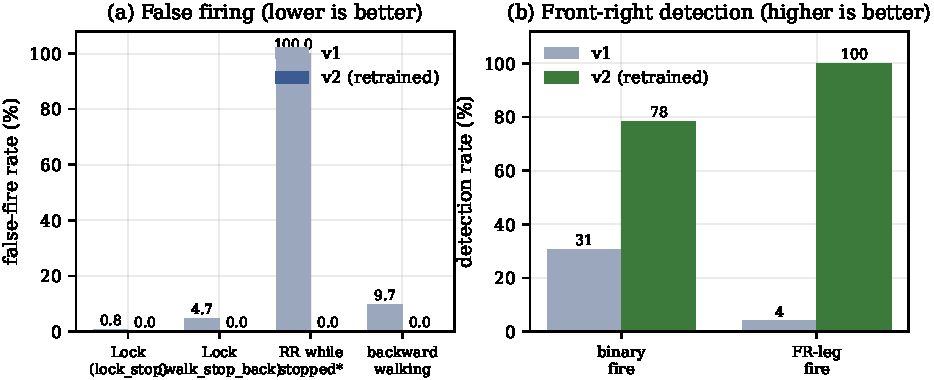
\includegraphics[width=\textwidth]{field_issues.pdf}
  \caption{Before/after the second data round. (a) False-firing rates on the three
  false-positive failures fall to zero. (b) Front-right detection rises from near-zero
  to full detection. All values are per-phase firing percentages on the named
  recordings.}
  \label{fig:field}
\end{figure*}

\begin{figure*}[t]
  \centering
  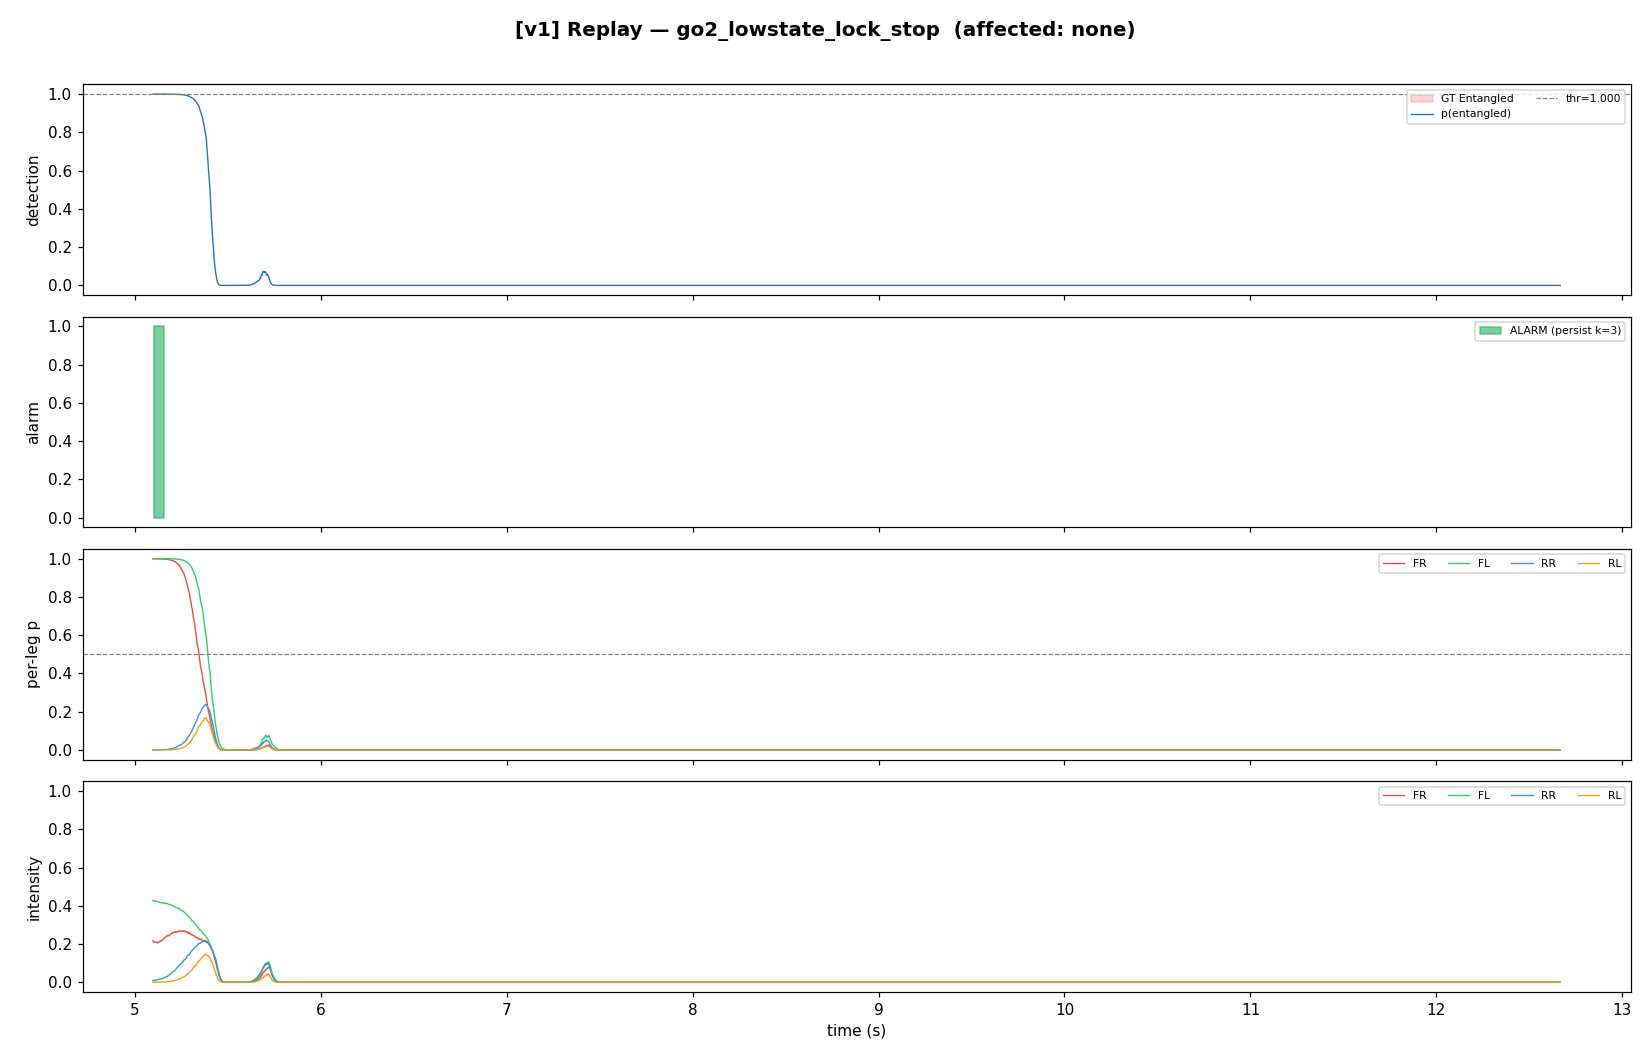
\includegraphics[width=0.94\textwidth]{lock_v1.png}\\[2pt]
  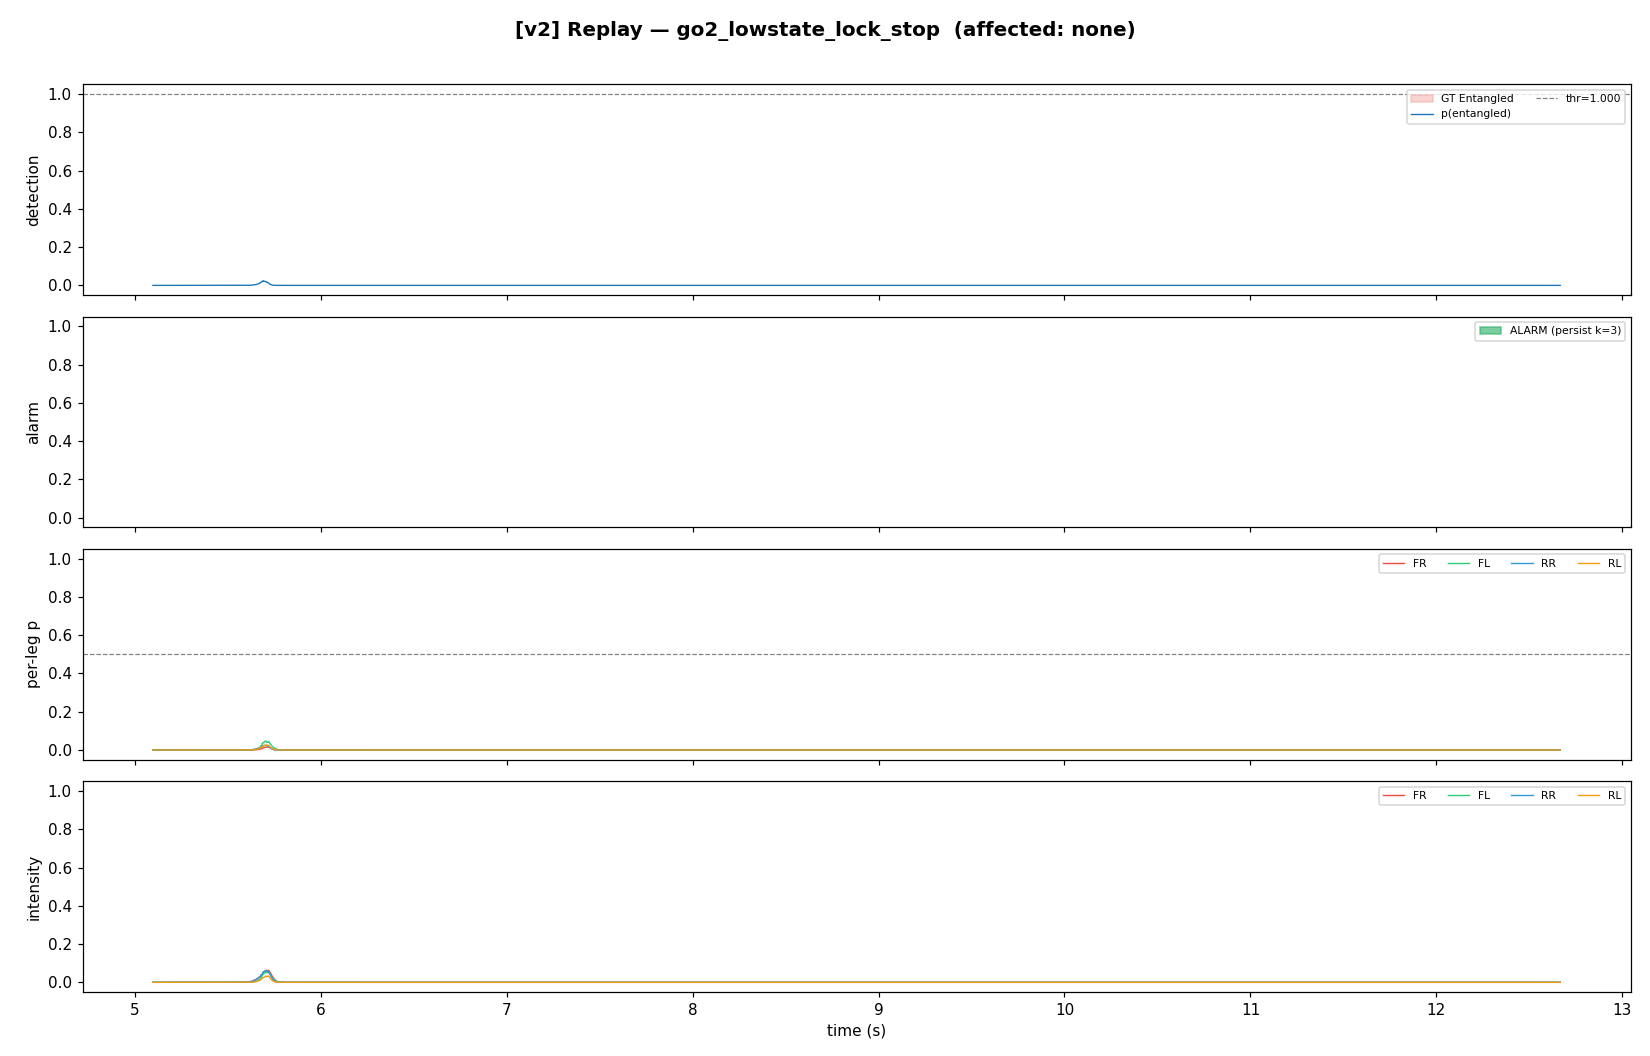
\includegraphics[width=0.94\textwidth]{lock_v2.png}
  \caption{Held-out \texttt{lock\_stop} recording (a pure stand-up-into-Lock negative)
  before (top) and after (bottom) the second data round. The post-stand-up firing is
  eliminated after training on \texttt{Lock} data.}
  \label{fig:lock}
\end{figure*}

\subsection{Runtime}
On a single CPU thread with the ONNX backend, per-window inference plus
post-processing takes a mean of $0.99$\,ms (median $0.95$\,ms, p95 $1.24$\,ms, max
$2.85$\,ms over $2{,}852$ windows), within the $2.0$\,ms budget at $500$\,Hz
(Fig.~\ref{fig:latency}, Table~\ref{tab:runtime}). The model is small
($\approx\!0.5$\,MB), so memory is dominated by the numpy buffers. If a target CPU is
slower than the budget, the node can decimate decisions without changing the window.

\begin{figure}[t]
  \centering
  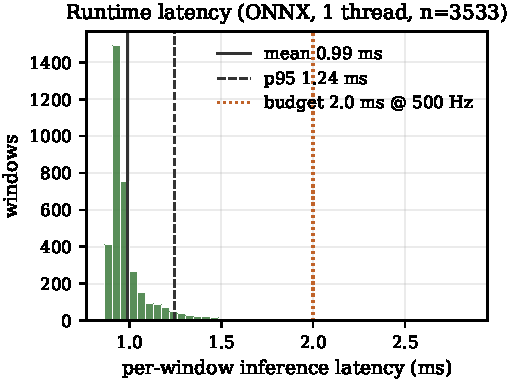
\includegraphics[width=0.9\columnwidth]{latency_hist.pdf}
  \caption{Per-window inference latency on one CPU thread (ONNX). The distribution
  sits well under the $2$\,ms real-time budget at $500$\,Hz.}
  \label{fig:latency}
\end{figure}

\begin{table}[t]
\centering
\caption{Runtime summary (single CPU thread, ONNX).}
\label{tab:runtime}
\small
\begin{tabular}{@{}lc@{}}
\toprule
Quantity & Value \\
\midrule
Mean / median latency & $0.99$ / $0.95$\,ms \\
p95 / max latency & $1.24$ / $2.85$\,ms \\
Real-time budget @ $500$\,Hz & $2.0$\,ms \\
Model size & $\approx\!0.5$\,MB \\
Runtime vs.\ research agreement & $\le 3.8\times10^{-7}$ \\
\bottomrule
\end{tabular}
\end{table}

\subsection{Recovery logic}
The recovery finite-state machine passes all $16$ unit tests and the plan runner all
$3$, covering the scenario matrix: normal walking, transient false alarms, a genuine
entanglement cycle, non-re-entrancy, the already-stopped shortcut, the fallen
escalation, command-failure faulting, verification failure and re-attempt, e-stop, and
reset. This verifies the \emph{logic}---the sequencing, gating, and safety
transitions---deterministically and without a robot.

\subsection{Verified results versus assumptions}
We are explicit about scope (Table~\ref{tab:assumptions}). \emph{Verified}: the
detection, calibration, ablation, and latency numbers above are offline results under
a leakage-safe protocol, and the deployment runtime matches the research pipeline to
$\approx\!10^{-6}$; the recovery logic is verified by unit tests. \emph{Assumptions
pending real-robot trials}: whether a given recovery motion actually frees a snagged
leg, and the chosen motion directions, magnitudes, and the weight-shift sign
convention, are engineering hypotheses grounded in mechanics but not yet measured on
hardware. For this reason the recovery layer ships with actuation disabled. We do not
claim recovery success rates, because we have not run actuated hardware trials.

\begin{table}[t]
\centering
\caption{Scope of claims.}
\label{tab:assumptions}
\small
\begin{tabular}{@{}p{0.60\columnwidth}p{0.30\columnwidth}@{}}
\toprule
Claim & Status \\
\midrule
Detection / attribution / calibration metrics & verified (offline, leakage-safe) \\
Runtime latency and real-time budget & verified (measured) \\
Research$\leftrightarrow$deployment numerical equivalence & verified ($\le\!10^{-6}$) \\
Recovery FSM sequencing / safety logic & verified (unit tests) \\
Recovery motion \emph{disentangles} a leg & assumption \\
Motion directions / magnitudes / weight-shift sign & assumption \\
Live-loop detector behavior on robot CPU/DDS & to be validated \\
\bottomrule
\end{tabular}
\end{table}

\section{Discussion and Limitations}
The main limitation is data scale and balance: $15$ positive events, with the
front-right leg in only three recordings, drive both the front-right precision
trade-off and the LORO variance. Collecting more front-right and front-both
interactions is the single highest-value next step. A second limitation is inherent to
the high-level API choice: the Sport-Mode interface keeps the robot within its own
balance controller and is verifiable, but it cannot command the arbitrary per-joint
trajectory that might best extricate a firmly caught leg; a low-level extrication
primitive is future work and carries additional safety burden. Third, the severity
index, while well-behaved, is a calibrated proxy rather than a measured force, and the
calibration analysis shows temperature scaling improves ranking and de-saturation more
than exact calibration. Finally, the recovery layer's physical efficacy is unverified;
the natural progression is a staged hardware campaign---detector-only, recovery in
dry-run, then actuated bring-up with an operator e-stop---feeding measured
disentanglement rates back into the strategy policy.

\section{Conclusion}
We presented a proprioception-only system that detects leg entanglement on a Unitree
Go2, localizes it to a leg, and estimates its severity, using a compact multi-task
causal TCN that runs in about a millisecond per window on a single CPU thread and
transfers from research to robot without a reimplementation gap. On leave-one-recording-out
cross-validation the detector reaches F1$=0.807\pm0.142$ and clearly outperforms a
rule-based baseline, and a targeted second data round removed four field-observed
failure modes at a small, documented cost. We coupled the detector to a safety-gated,
detector-aware recovery state machine that selects among verified high-level motions in
a closed loop, and we verified its logic in simulation while being explicit that the
physical disentanglement efficacy remains to be measured on hardware. We believe the
combination of per-leg attribution, label-free severity estimation, and a decoupled,
verifiable recovery layer is a useful template for turning a subtle proprioceptive
fault into an actionable, real-time signal.

\bibliographystyle{IEEEtran}
\bibliography{references}

\appendix
\begin{figure*}[t]
  \centering
  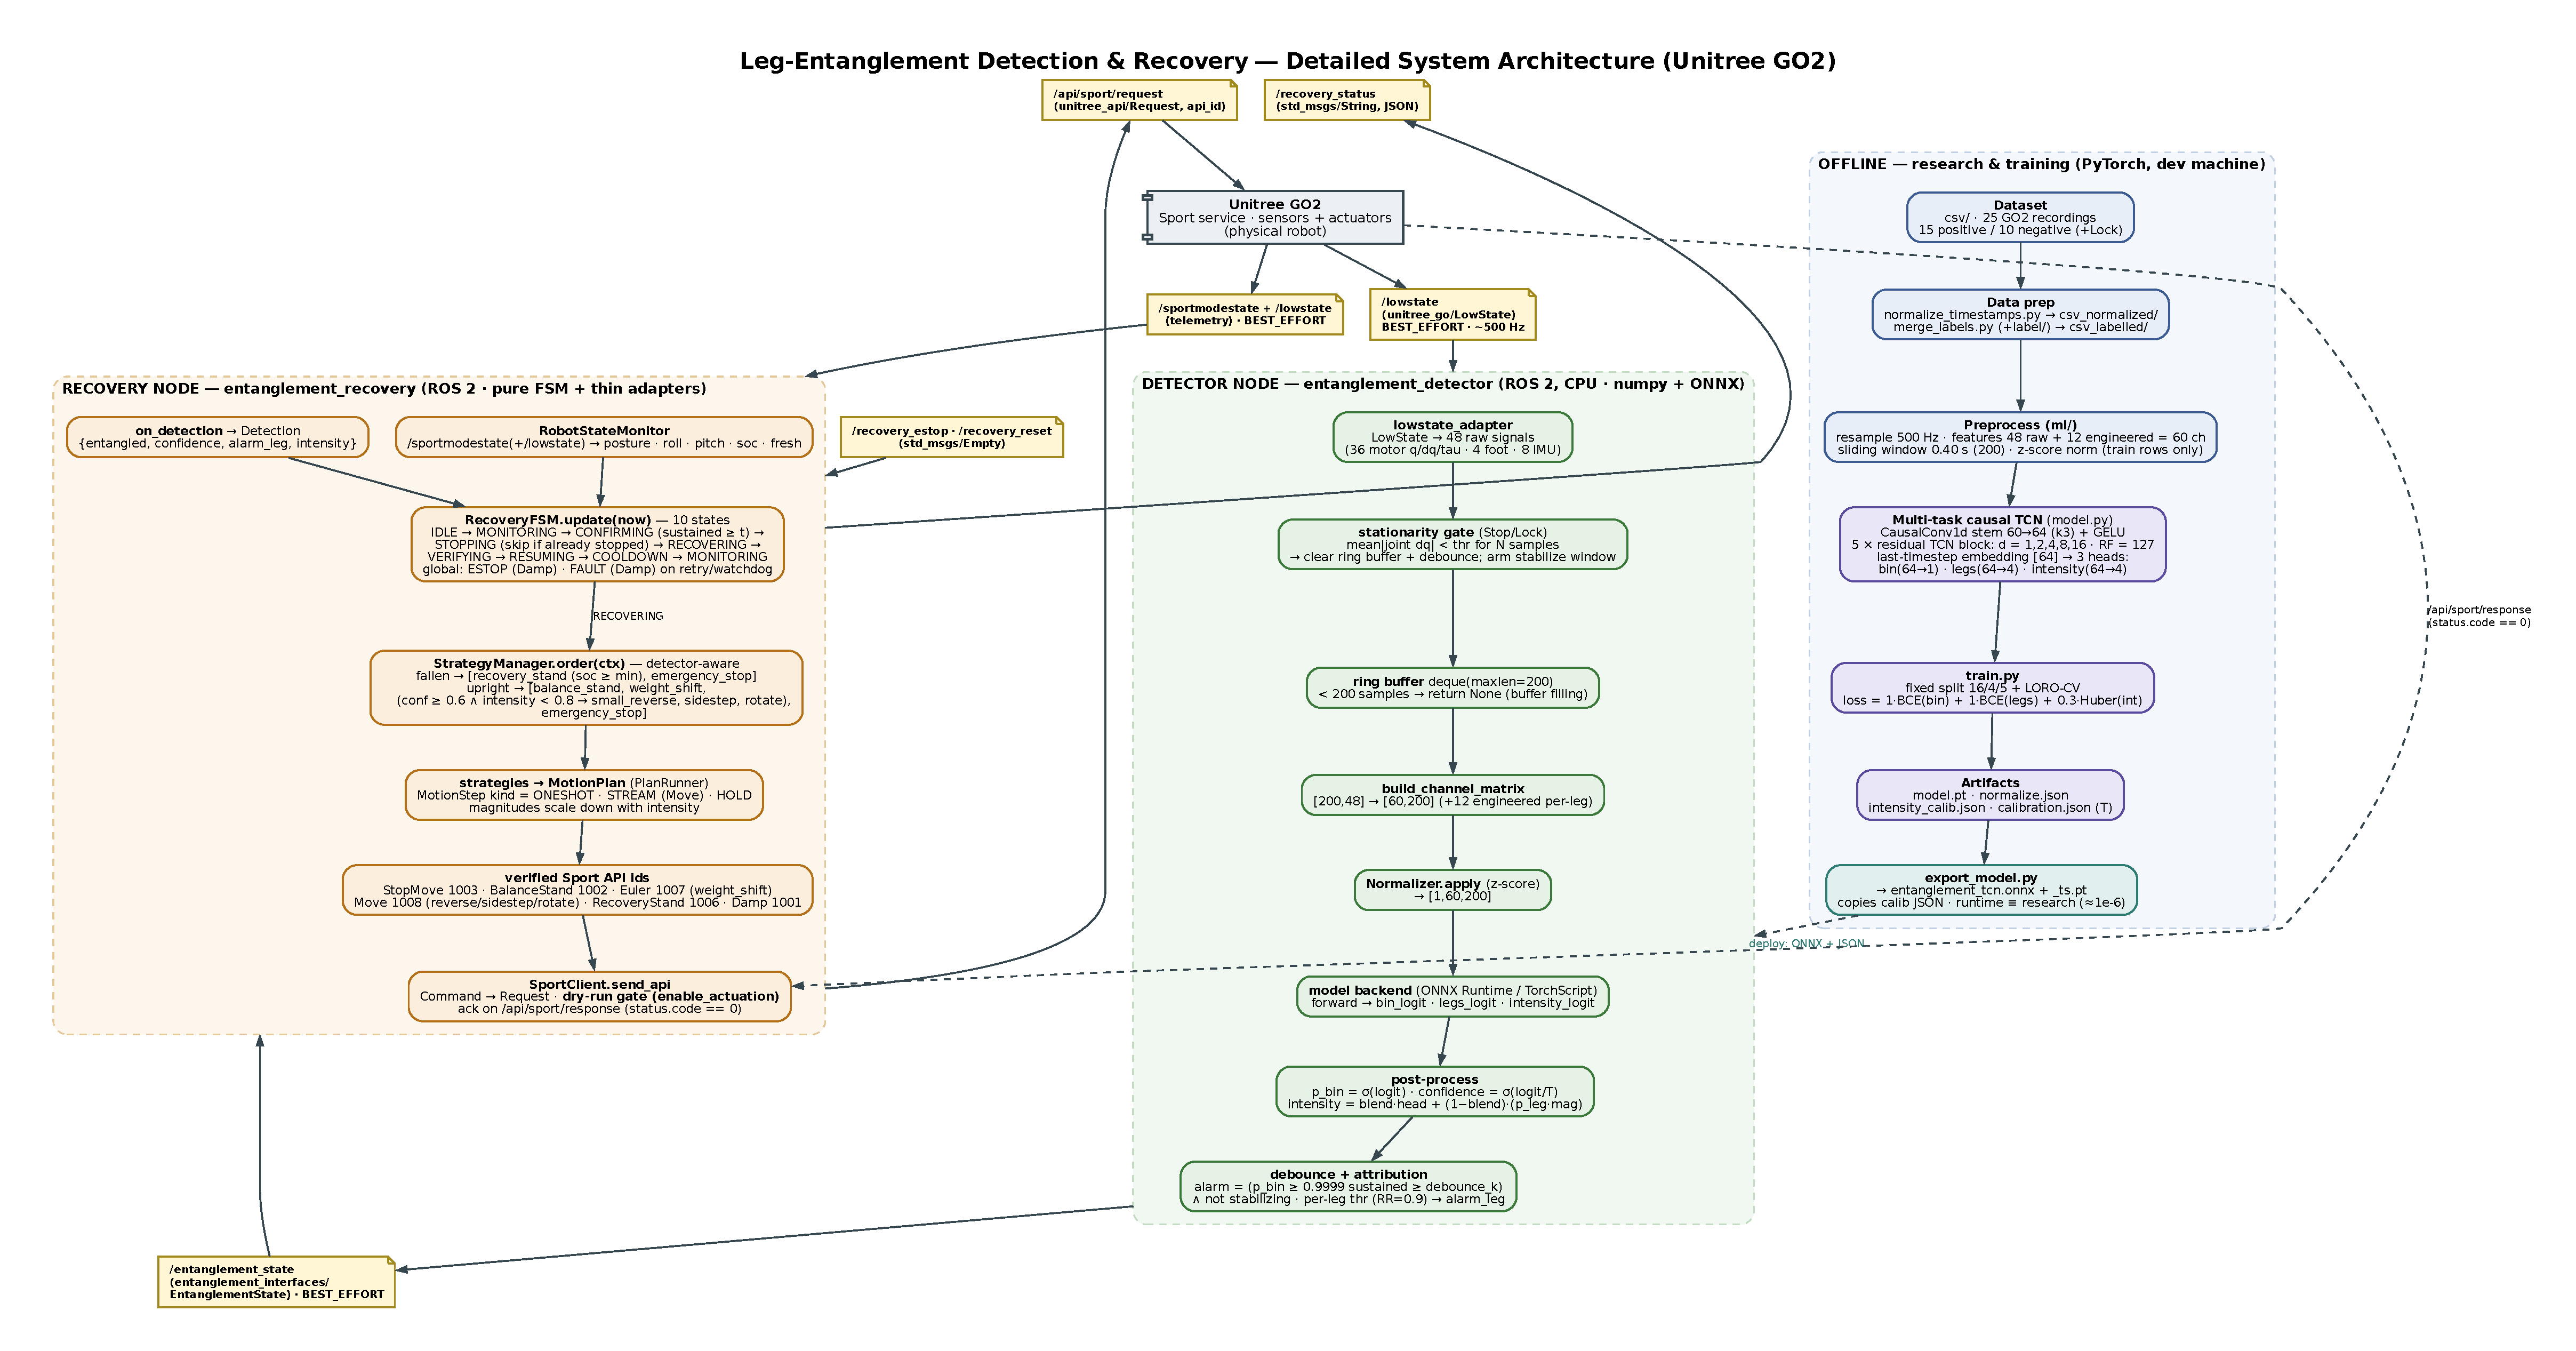
\includegraphics[width=\textwidth]{architecture_detailed.pdf}
  \caption{Detailed architecture (appendix). Every processing block, ROS\,2 topic with
  message type and QoS, the ten-state recovery machine, the detector-aware strategy
  ordering, and the verified Sport-API identifiers, matching the implementation.}
  \label{fig:detailed}
\end{figure*}

\end{document}
